\documentclass[conference]{IEEEtran}
\IEEEoverridecommandlockouts

\usepackage{cite}
\usepackage{amsmath,amssymb}
\usepackage{graphicx}
\usepackage{booktabs}
\usepackage{multirow}
\usepackage{array}
\usepackage{url}
\usepackage{xcolor}
\usepackage{balance}
\usepackage{enumitem}
\usepackage[hidelinks]{hyperref}
\usepackage{dblfloatfix}

\newcommand{\method}{BOPS}
\newcommand{\datasetocr}{TextOCR}
\newcommand{\datasetvlm}{DocVQA}

\begin{document}

\title{When Text-Aware Patching Helps and Fails:\\
A Budget-Aware Study of OCR Preservation and VLM Evidence Selection}

\author{\IEEEauthorblockN{Mohammad Rayaan Raza}
\IEEEauthorblockA{Department of Computer Science\\
National University of Computer and Emerging Sciences (FAST-NUCES)\\
Islamabad, Pakistan\\
Email: 23I-0535@nu.edu.pk}
}

\maketitle

\begin{abstract}
Text-rich images such as documents, receipts, screenshots, forms, and slides often exceed practical resolution, byte, or visual-token budgets for optical character recognition (OCR) systems and vision-language models (VLMs). Common preprocessing strategies such as resizing and compression reduce input cost, but can remove small text or distort evidence needed for downstream reasoning. This paper presents a budget-aware empirical study of preprocessing strategies for text-rich image understanding. We compare area-based resizing, byte-budget JPEG/WebP compression, overview-only reduction, random and uniform patching, and a training-free OCR-guided overview-plus-patch method, \method. \method{} provides a low-resolution overview together with $K$ high-resolution patches selected using OCR-derived text coverage, OCR confidence, edge density, and entropy. On a 200-image \datasetocr{} evaluation, \method{} with eight patches improves OCR word recall over aggressive resizing at area ratio 0.25, with a paired bootstrap mean difference of $+0.077$ and 95\% CI $[+0.052,+0.102]$. However, on a 100-question \datasetvlm{} evaluation using Qwen2.5-VL-3B, \method{} does not significantly improve VLM question answering over random or uniform patching and remains far below the resized full-image baseline. Post-hoc diagnostics show that ground-truth answers appear in full-image OCR for 76\% of \method{} cases but in selected-patch OCR for only 6\%. The results indicate that OCR-guided patching can preserve text under strict spatial budgets, but question-agnostic text-density selection is insufficient for document VQA. The central lesson is that OCR preservation and answer-evidence preservation are related but not equivalent.
\end{abstract}

\begin{IEEEkeywords}
OCR, document image understanding, vision-language models, visual budgets, patch selection, DocVQA, TextOCR, image compression.
\end{IEEEkeywords}

\section{Introduction}
Text-rich visual inputs are common in practical multimodal systems: scanned documents, receipts, screenshots, forms, slides, tables, infographics, posters, and scene-text images. Such images often contain small text and layout structure that can be destroyed by naive resizing. Full-resolution processing is expensive for OCR pipelines and modern VLMs, while byte-level compression does not necessarily reduce the number of visual tokens processed by a VLM. This creates a practical tension: reducing input cost can damage the exact text and spatial evidence needed for OCR and document question answering.

Recent document understanding models combine text, layout, and visual cues at model level \cite{layoutlm,layoutlmv2,layoutlmv3,docformer,tilt,udop,donut,pix2struct}, while high-resolution VLM methods increasingly rely on dynamic resolution, patching, or token-efficient visual processing \cite{navit,llavauhd,qwen25vl}. In contrast, this work studies a simpler but under-examined question: before changing or retraining the downstream model, how much can input-side preprocessing preserve useful text evidence under declared budgets?

We study this question through a training-free preprocessing strategy called \method{}: Budget-Aware OCR-Guided Overview-Plus-Patch Selection. \method{} sends a low-resolution overview of the full image plus a small number of high-resolution OCR-guided patches. The overview preserves approximate global layout, while patches preserve local text detail. The method is intentionally simple: it is designed not as a new OCR engine or VLM, but as a controlled probe for understanding when text-aware patch selection helps and when it fails.

\textbf{Research questions.} We structure the paper around four questions:
\begin{itemize}[leftmargin=*]
    \item \textbf{RQ1:} How do resizing, byte compression, and patch-based representations affect OCR word recall under declared visual budgets?
    \item \textbf{RQ2:} Does OCR-guided patch selection preserve more OCR signal than aggressive spatial resizing?
    \item \textbf{RQ3:} Does improved OCR preservation transfer to VLM question-answering performance?
    \item \textbf{RQ4:} When VLM patching fails, is the bottleneck OCR visibility, patch selection, or VLM reasoning?
\end{itemize}

\textbf{Contributions.} This paper makes four contributions:
\begin{enumerate}[leftmargin=*]
    \item A budget-aware evaluation protocol comparing resizing, byte compression, overview-only input, random patches, uniform patches, and OCR-guided patches.
    \item A training-free OCR-guided overview-plus-patch preprocessing method that selects high-resolution regions without modifying the downstream OCR or VLM.
    \item A controlled OCR evaluation showing that OCR-guided patches significantly improve word recall over aggressive resizing, while JPEG/WebP remain strong baselines.
    \item A failure analysis showing that OCR-preserving patch selection does not necessarily preserve answer-bearing evidence for DocVQA, motivating question-aware selection.
\end{enumerate}

\section{Related Work}
\subsection{Text-Rich Image Benchmarks}
\datasetocr{} provides large-scale arbitrary-shaped scene-text annotations on real images and is designed to isolate OCR performance in settings where scene text is important for reasoning \cite{textocr}. \datasetvlm{} evaluates visual question answering over document images and tests whether systems can locate and reason over document evidence \cite{docvqa}. OCR-centric VLM benchmarks such as OCRBench and OCRBench v2 further show that visual text localization and reasoning remain difficult for modern multimodal models \cite{ocrbenchv2}.

\subsection{Document Understanding Models}
Document AI models have increasingly integrated text, layout, and image information. LayoutLM introduced joint modeling of text and layout for scanned document understanding \cite{layoutlm}. LayoutLMv2 and LayoutLMv3 extended this line with stronger multimodal pretraining and word-patch alignment objectives \cite{layoutlmv2,layoutlmv3}. DocFormer, TILT, and UDOP similarly emphasize the role of layout-aware multimodal representations \cite{docformer,tilt,udop}. OCR-free models such as Donut and Pix2Struct avoid explicit OCR pipelines and directly map document-like images to structured text outputs \cite{donut,pix2struct}. Unlike these model-side approaches, this paper studies preprocessing before OCR or VLM inference.

\subsection{High-Resolution and Token-Efficient Vision-Language Models}
High-resolution image understanding is challenging because fixed-size resizing can remove fine details. NaViT explores native-resolution ViTs with sequence packing to avoid fixed resizing \cite{navit}. LLaVA-UHD uses modularized high-resolution slices and a compression module for efficient large multimodal model inference \cite{llavauhd}. Qwen2.5-VL supports dynamic visual processing and document parsing capabilities \cite{qwen25vl}. Visual-token pruning work further targets inference efficiency by removing redundant tokens after visual encoding \cite{adaptiveprune,divprune}. In contrast, \method{} is an input-side method: it selects image regions before downstream model encoding.

\subsection{Compression and Machine Reading}
JPEG and WebP are practical baselines because they reduce file size while often preserving visual readability \cite{jpeg,webp}. However, byte compression and visual-token cost are not identical. A compressed image may still be internally resized or tokenized by the VLM into a large visual sequence. Therefore, this paper reports byte utilization for JPEG/WebP and treats compression as a strong practical baseline rather than a direct proxy for VLM token reduction.

\section{Method}
\subsection{Budget Model}
Each preprocessing method declares a budget axis: pixel area for resizing, byte size for JPEG/WebP, and patch count for patch-based methods. Method--budget pairs that are semantically incompatible are marked \emph{not applicable} and excluded from aggregates. Attempted transformations that miss their declared budget are marked \emph{invalid} and excluded. Pixel budgets use a $\pm3\%$ tolerance around the target area. Byte-budget methods are valid when the actual encoded size is at or below the target; byte utilization is reported. Patch budgets require exactly $K$ selected patches.

This design prevents empty or unfair cross-axis comparisons, e.g., JPEG is not evaluated under an area budget and BOPS is not evaluated under a byte budget. For clarity, results tables report each method under its own declared budget axis.

\subsection{Baselines}
We compare the following methods:
\begin{itemize}[leftmargin=*]
    \item \textbf{Original:} full-resolution reference image.
    \item \textbf{Resize:} uniform area-ratio scaling.
    \item \textbf{JPEG/WebP:} byte-budget compression with actual size at or below target.
    \item \textbf{Overview-only:} low-resolution global image only.
    \item \textbf{Random patches:} overview plus randomly sampled high-resolution patches.
    \item \textbf{Uniform patches:} overview plus evenly spaced high-resolution patches.
\end{itemize}

\subsection{BOPS: Budget-Aware OCR-Guided Patch Selection}
Given an input image, \method{} generates a low-resolution overview and a grid of candidate high-resolution patches. OCR is run on the original image to obtain text boxes and confidence scores. Candidate patches are scored by:
\begin{equation}
    s(p) = 0.40C_{text}(p) + 0.30C_{conf}(p) + 0.15E(p) + 0.15H(p),
\end{equation}
where $C_{text}$ is OCR text-box coverage, $C_{conf}$ is mean OCR confidence of overlapping text boxes, $E$ is edge density, and $H$ is entropy. Non-maximum suppression removes redundant high-overlap patches, and the top $K$ patches are selected. Fig.~\ref{fig:pipeline} summarizes the pipeline.

\begin{figure*}[!ht]
    \centering
    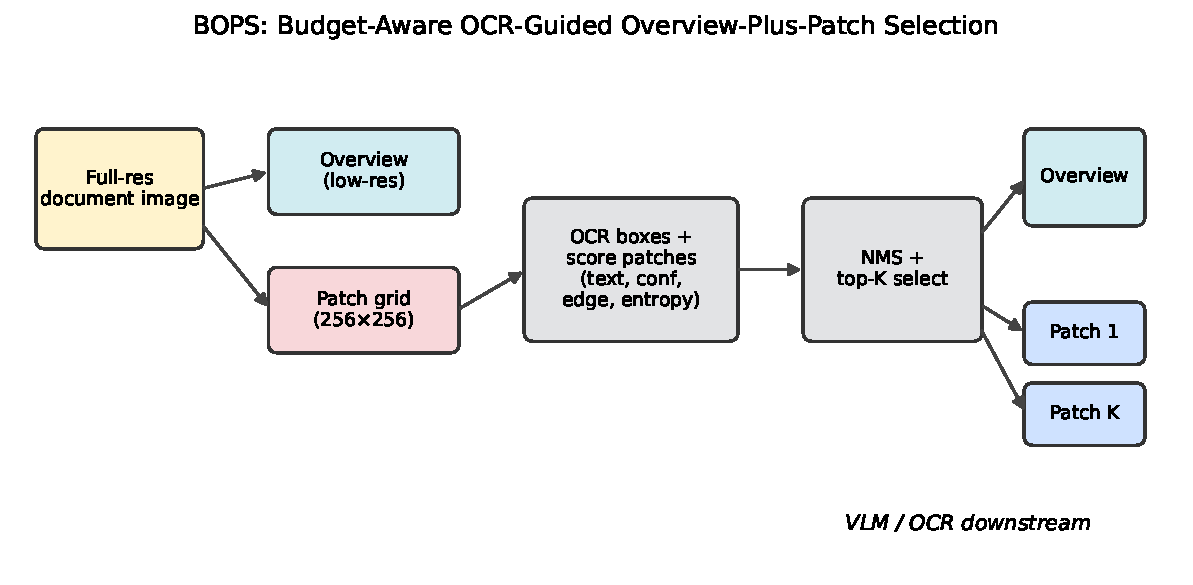
\includegraphics[width=0.93\textwidth]{figures/bops_pipeline.pdf}
    \caption{BOPS pipeline. The image is represented as one low-resolution overview plus $K$ high-resolution patches selected using OCR-derived and image-statistical signals.}
    \label{fig:pipeline}
\end{figure*}

For OCR evaluation, OCR is run on the overview and selected patches, and recognized text is merged. For VLM evaluation, the overview and selected patches are passed as multi-image input. Ground-truth answers are never used for patch selection; they are used only for post-hoc diagnostics.

\subsection{Question-Aware BOPS}
We also evaluate a question-aware variant that uses only the DocVQA question (never the ground-truth answer). Candidate patches are re-scored as
\begin{equation}
\begin{split}
    s_q(p) = {} & 0.30C_{text}(p) + 0.20C_{conf}(p) + 0.25O_q(p) \\
                & + 0.15S_q(p) + 0.05E(p) + 0.05H(p),
\end{split}
\end{equation}
where $O_q$ is question-token overlap with OCR text inside the patch and $S_q$ is normalized string similarity between the question and patch OCR text.

\section{Experimental Setup}
\subsection{Datasets and Scale}
The OCR track uses a 200-image \datasetocr{} sample. The VLM track uses 100 \datasetvlm{} questions. These pilot-scale experiments are sufficient for controlled analysis but are not a full benchmark replacement. The repository uses manifest files to ensure that each image/question is evaluated consistently across methods.

\subsection{Backends}
OCR is performed using EasyOCR with GPU acceleration when CUDA is available. VLM inference uses Qwen2.5-VL-3B-Instruct in 4-bit quantization on an RTX 3050 Laptop GPU. The VLM prompt is fixed across methods; single-image methods receive one image, while patch methods receive the overview followed by selected patches.

\subsection{Metrics and Statistical Testing}
OCR is evaluated using character error rate (CER), word error rate (WER), count-aware word recall, word precision, word F1, predicted-token count, and duplicate-token ratio. Word recall measures how much ground-truth text is recovered; word precision measures how much of the predicted text is correct. Together they distinguish genuine recognition gains from verbose OCR merging. VLM QA is evaluated using exact match (EM) and ANLS. We compute paired bootstrap confidence intervals for the main OCR and VLM comparisons.

\section{Results}
\subsection{RQ1--RQ2: OCR Preservation Under Budget}
Table~\ref{tab:ocr} summarizes the OCR results. Aggressive resizing reduces word recall: resize at area ratio 0.25 obtains 0.163 compared with 0.275 for the original image. \method{} improves monotonically with patch count: patches 2, 4, and 8 obtain word recall 0.172, 0.204, and 0.240 respectively. The paired bootstrap comparison in Table~\ref{tab:ci} shows that \method{} with eight patches improves word recall over resize at area 0.25 by $+0.077$ with 95\% CI $[+0.052,+0.102]$.

However, JPEG/WebP remain strong baselines. JPEG at 200 KB obtains word recall 0.274 and WebP at 200 KB obtains 0.273, both close to original and higher than \method{} patches 8. Thus, the defensible OCR claim is not that \method{} beats all preprocessing methods; rather, it improves over aggressive spatial downscaling.

\textbf{Precision vs.\ verbosity.} Table~\ref{tab:ocr_precision} shows that \method{} increases word recall over resize at area 0.25 (0.240 vs.\ 0.163) but lowers word precision (0.217 vs.\ 0.296). Word F1 is nearly unchanged (0.199 vs.\ 0.193), and CER/WER worsen because patch merging introduces extra OCR text. The gain is therefore better \emph{coverage} of ground-truth tokens, not uniformly cleaner recognition. Fig.~\ref{fig:ocr_recall} visualizes the recall trend.

\begin{figure}[!ht]
    \centering
    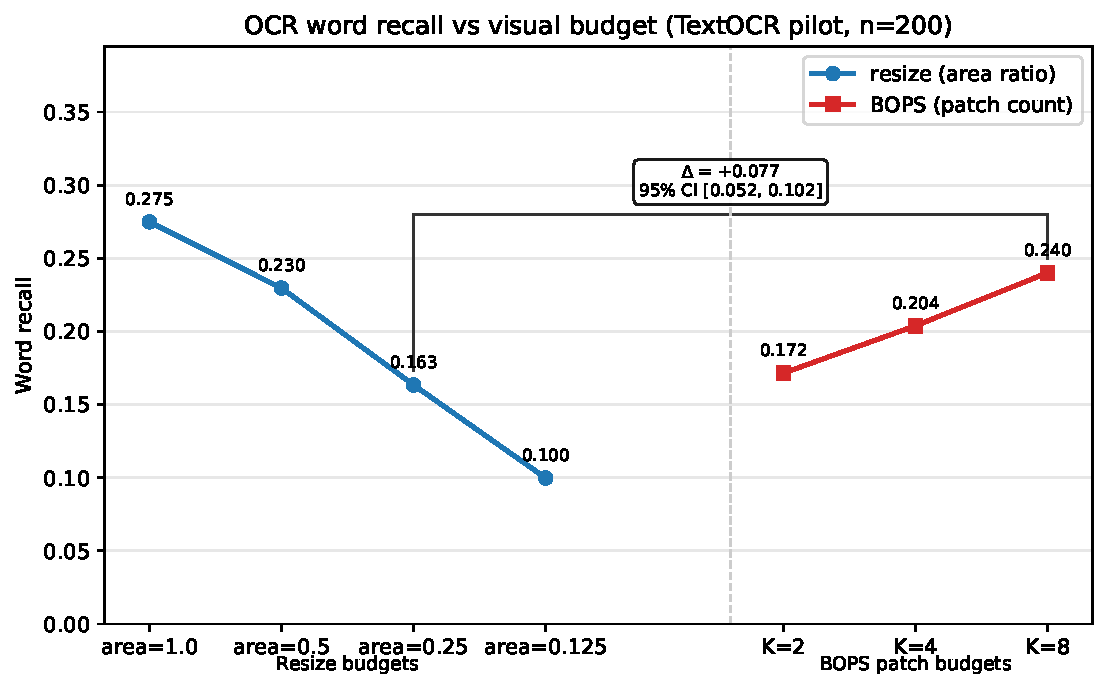
\includegraphics[width=\columnwidth]{figures/ocr_word_recall_budget.pdf}
    \caption{OCR word recall on \datasetocr{} (n=200). BOPS improves with patch count and outperforms resize at area 0.25, but remains below the original image.}
    \label{fig:ocr_recall}
\end{figure}

\begin{table}[!ht]
\centering
\caption{OCR precision analysis at key budgets (TextOCR pilot, $n{=}200$).}
\label{tab:ocr_precision}
\begin{tabular}{llcccc}
\toprule
Method & Budget & Recall & Prec. & F1 & CER \\
\midrule
resize & area\_0.25 & 0.163 & 0.296 & 0.193 & 0.752 \\
bops & patches\_8 & 0.240 & 0.217 & 0.199 & 1.021 \\
jpeg & kb\_200 & 0.274 & 0.380 & 0.301 & 0.680 \\
\bottomrule
\end{tabular}
\end{table}

\begin{table*}[!ht]
\centering
\caption{OCR results on \datasetocr{} (n=200). Word recall is primary. Byte utilization is reported only for JPEG/WebP.}
\label{tab:ocr}
\begin{tabular}{llccccc}
\toprule
Method & Budget & Word recall & CER & WER & n & Byte util. \\
\midrule
original & area\_1.0 & 0.275 & 0.674 & 0.883 & 200 & -- \\
resize & area\_0.5 & 0.230 & 0.685 & 0.861 & 200 & -- \\
resize & area\_0.25 & 0.163 & 0.752 & 0.901 & 200 & -- \\
resize & area\_0.125 & 0.100 & 0.822 & 0.921 & 200 & -- \\
jpeg & kb\_500 & 0.275 & 0.677 & 0.888 & 200 & 0.39 \\
jpeg & kb\_200 & 0.274 & 0.680 & 0.886 & 200 & 0.83 \\
jpeg & kb\_100 & 0.261 & 0.677 & 0.885 & 199 & 0.97 \\
jpeg & kb\_50 & 0.245 & 0.689 & 0.879 & 199 & 0.98 \\
webp & kb\_500 & 0.273 & 0.673 & 0.877 & 200 & 0.34 \\
webp & kb\_200 & 0.273 & 0.675 & 0.878 & 200 & 0.76 \\
webp & kb\_100 & 0.269 & 0.675 & 0.882 & 199 & 0.93 \\
webp & kb\_50 & 0.257 & 0.687 & 0.897 & 199 & 0.98 \\
bops & patches\_2 & 0.172 & 0.822 & 1.030 & 200 & -- \\
bops & patches\_4 & 0.204 & 0.904 & 1.198 & 200 & -- \\
bops & patches\_8 & 0.240 & 1.021 & 1.426 & 200 & -- \\
\bottomrule
\end{tabular}
\end{table*}

\subsection{RQ3: Transfer to VLM Question Answering}
Table~\ref{tab:vlm} and Fig.~\ref{fig:vlm} show that OCR preservation does not transfer to VLM QA. Resize dominates the DocVQA pilot with ANLS 0.788 and EM 0.680. \method{} obtains ANLS 0.193, close to overview-only (0.190) and random patches (0.157), but below uniform patching (0.212). The paired CI for \method{} versus random crosses zero, so the mean improvement over random should not be interpreted as significant.

This result changes the interpretation of \method{}. The method is useful as a probe and an OCR-preserving spatial-budget strategy, but the current question-agnostic scoring is not sufficient for VLM evidence selection.

We also evaluated question-aware \method{} (\texttt{bops\_qa}), which reweights patches using question-token overlap and question--patch OCR similarity (no ground-truth answer). On the same 100-question pilot, \texttt{bops\_qa} improves mean ANLS from 0.193 to 0.225 and EM from 0.14 to 0.15 versus default \method{}, but selected-patch answer coverage remains 5\% (vs.\ 6\% for default \method{}). The VLM gain is modest and patch selection is still the bottleneck; resize remains far stronger (ANLS 0.788). Fig.~\ref{fig:vlm} compares all methods.

\begin{figure}[!ht]
    \centering
    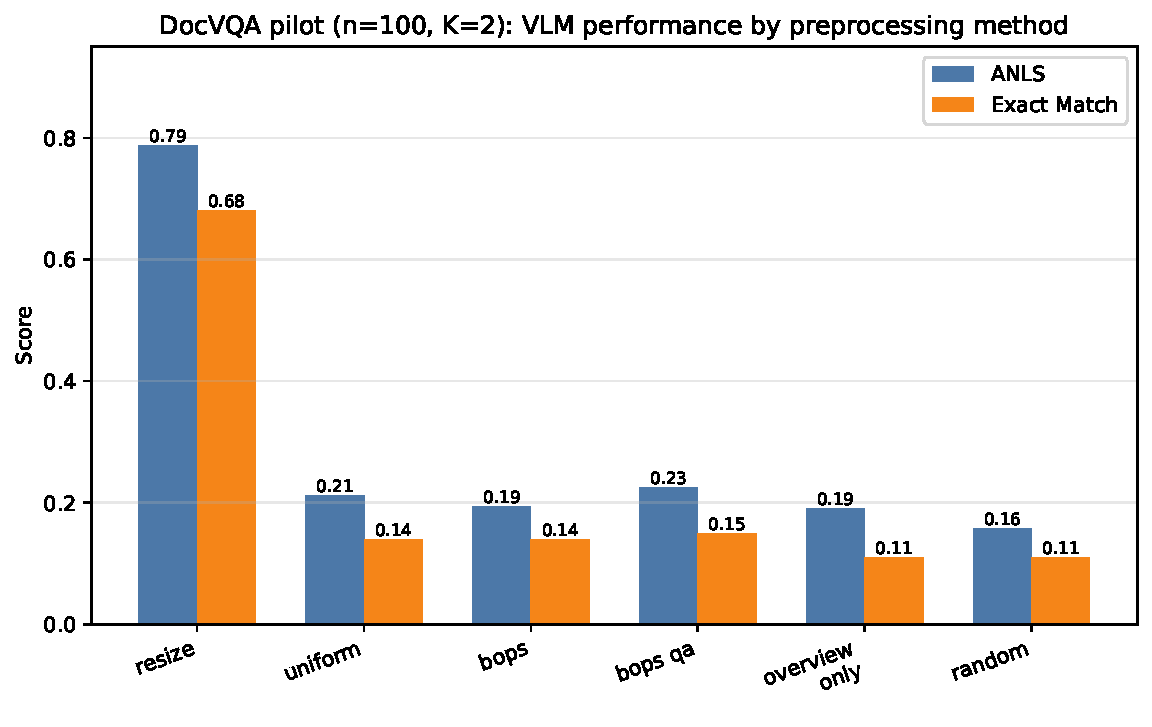
\includegraphics[width=\columnwidth]{figures/vlm_anls_methods.pdf}
    \caption{DocVQA performance (n=100, K=2), including question-aware \texttt{bops\_qa}. Resize dominates; patch methods remain far below resize.}
    \label{fig:vlm}
\end{figure}

\begin{table}[!ht]
\centering
\caption{DocVQA pilot results (n=100, K=2).}
\label{tab:vlm}
\begin{tabular}{lccc}
\toprule
Method & EM & ANLS & n \\
\midrule
resize & 0.680 & 0.788 & 100 \\
uniform & 0.140 & 0.212 & 100 \\
bops & 0.140 & 0.193 & 100 \\
bops\_qa & 0.150 & 0.225 & 100 \\
overview-only & 0.110 & 0.190 & 100 \\
random & 0.110 & 0.157 & 100 \\
\bottomrule
\end{tabular}
\end{table}

\subsection{RQ4: Failure Diagnosis}
Post-hoc diagnostics reveal the central failure mode. For all patch-based methods, the ground-truth answer appears in full-image OCR for about 76\% of samples, but appears in selected-patch OCR for only 0--6\% (Fig.~\ref{fig:coverage}). Random (3\%) and uniform (2\%) are no better than default \method{} (6\%) or question-aware \method{} (5\%); overview-only necessarily scores 0\% on patch OCR. This means the VLM often never receives the answer-bearing region regardless of selector, and $K{=}2$ is severely budget-limited.

The problem is therefore not only language reasoning; it is evidence selection. Dense text regions can score highly under OCR coverage and confidence while the answer may be a small field such as a date, amount, name, or form value. Fig.~\ref{fig:coverage} compares answer coverage across patch selectors, and Fig.~\ref{fig:failures} shows one representative failure case at publication scale; additional examples appear in the appendix.

\begin{figure}[!ht]
    \centering
    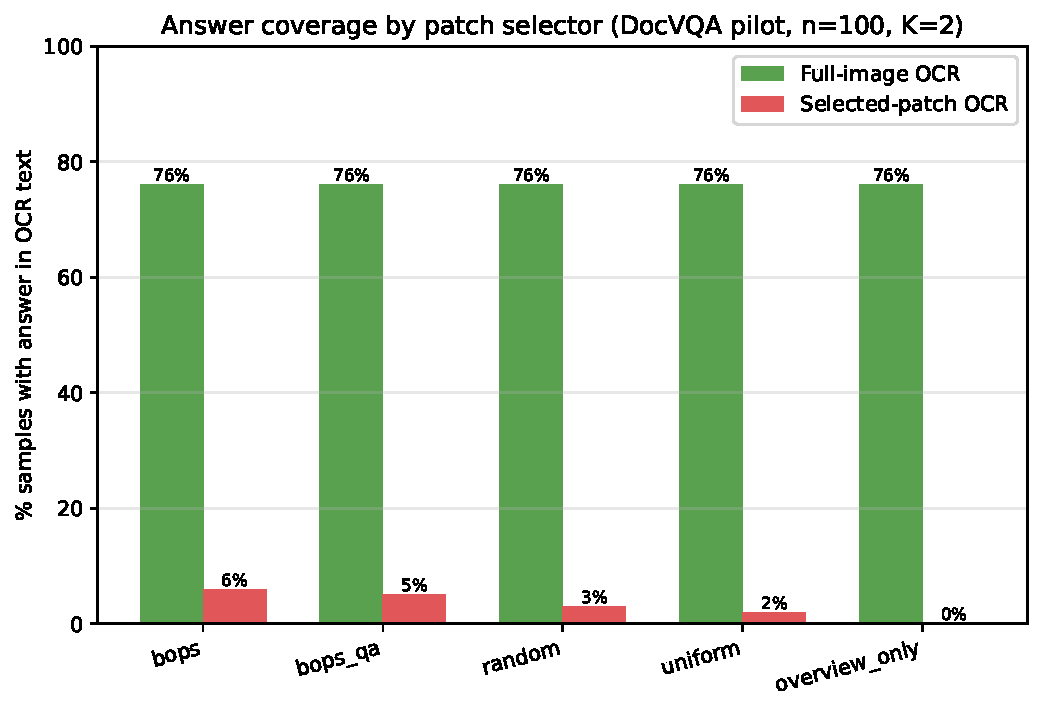
\includegraphics[width=\columnwidth]{figures/answer_coverage_diagnostics.pdf}
    \caption{Answer coverage by patch selector (DocVQA, $n{=}100$, $K{=}2$). Full-image OCR contains the answer far more often than selected-patch OCR for every patch method.}
    \label{fig:coverage}
\end{figure}

\begin{figure*}[!ht]
    \centering
    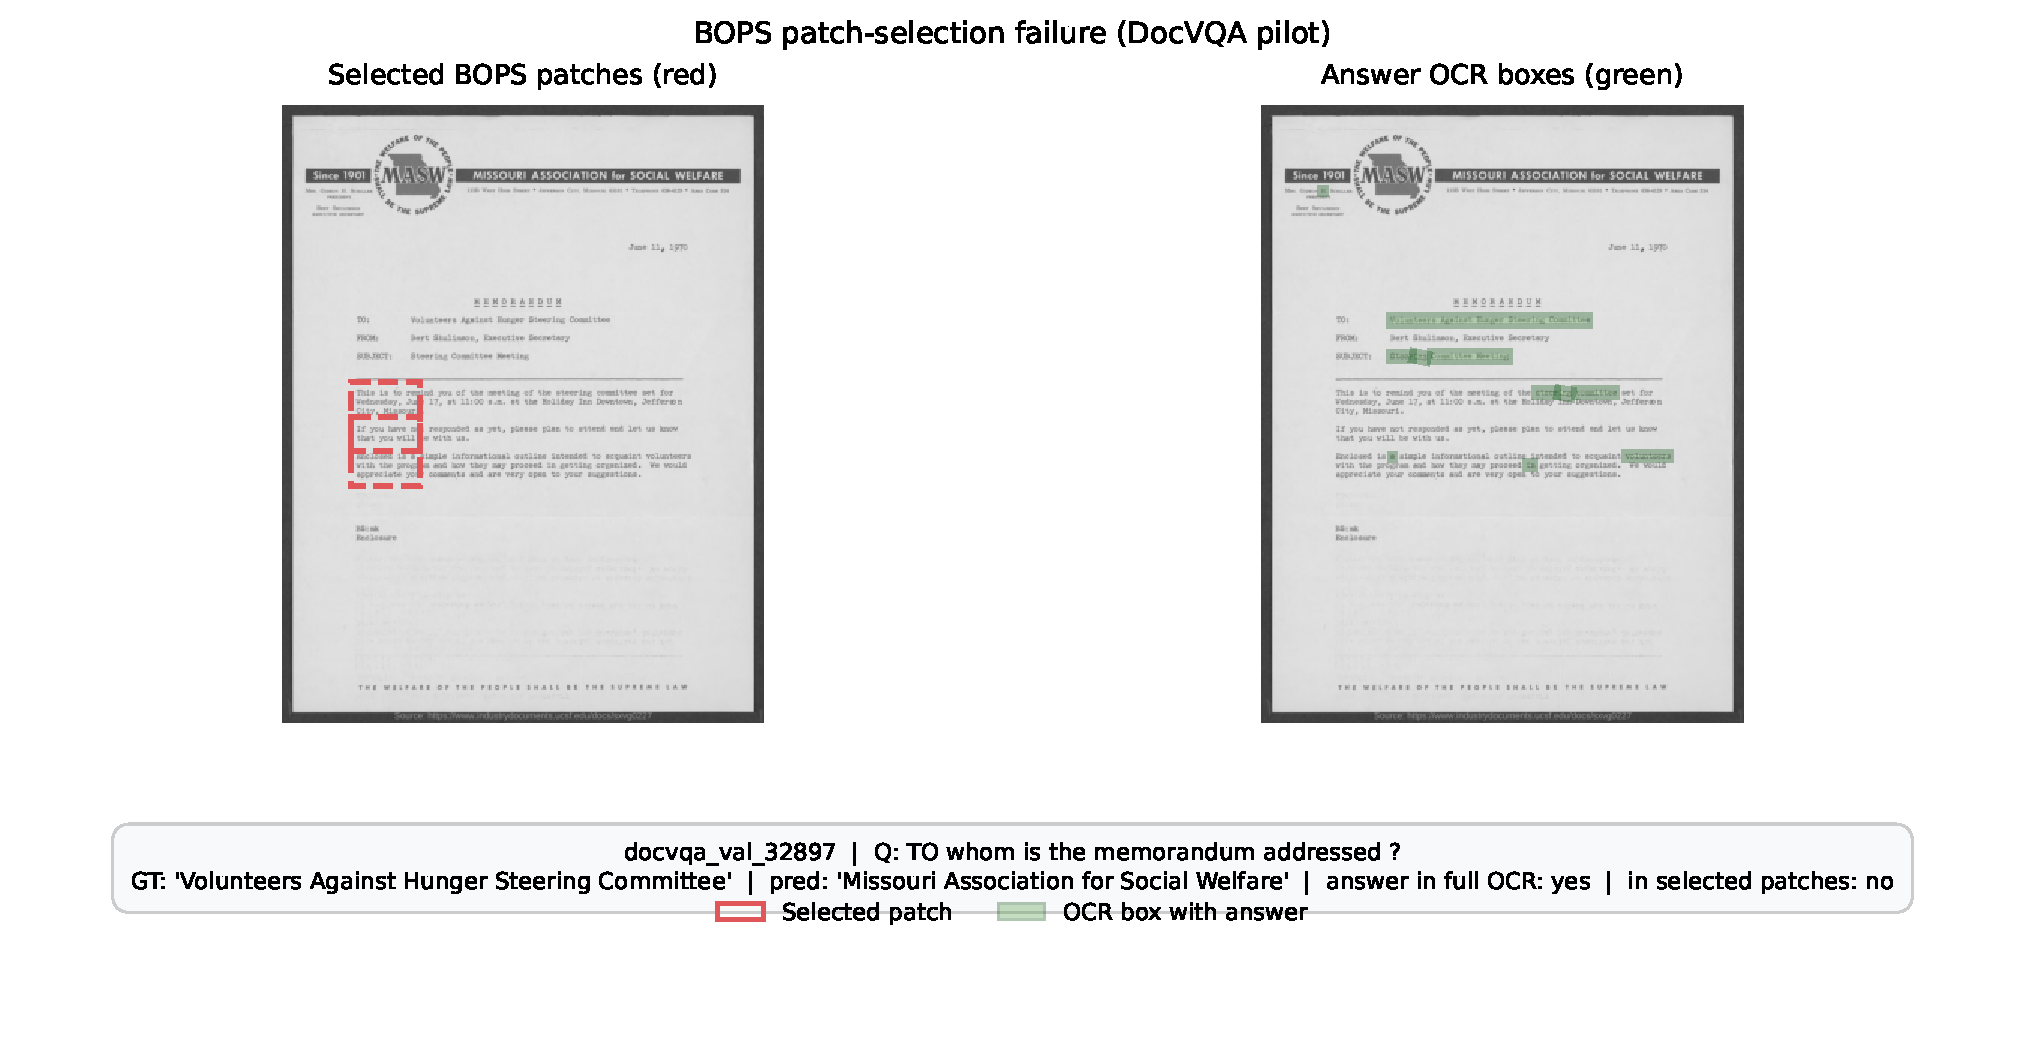
\includegraphics[width=\textwidth]{figures/failure_panel.pdf}
    \caption{Representative DocVQA failure (one example). Selected \method{} patches (red) miss answer-bearing OCR regions (green) even though the answer is visible in full-image OCR.}
    \label{fig:failures}
\end{figure*}

\subsection{Efficiency and Budget Accounting}
Table~\ref{tab:budget} summarizes declared budgets and median runtime. \method{} uses more pixels than resize at area 0.25 (median 574k vs.\ 197k for patches 8 vs.\ area 0.25) and sends three images to the VLM (overview + 2 patches). Fig.~\ref{fig:runtime} shows the runtime cost: median VLM runtime is 20.9\,s for \method{} versus 2.5\,s for resize.

\begin{table}[!ht]
\centering
\caption{Budget and cost summary (pilot medians).}
\label{tab:budget}
\resizebox{\columnwidth}{!}{%
\begin{tabular}{llrrr}
\toprule
Track & Method & Pixels & VLM imgs & VLM $t$ (s) \\
\midrule
OCR & resize (a0.25) & 197k & -- & -- \\
OCR & bops (p8) & 574k & -- & -- \\
OCR & jpeg (kb200) & 189k & -- & -- \\
VLM & resize & -- & 1 & 2.5 \\
VLM & bops & -- & 3 & 20.9 \\
VLM & uniform & -- & 3 & 2.1 \\
\bottomrule
\end{tabular}}
\end{table}

\begin{figure}[!ht]
    \centering
    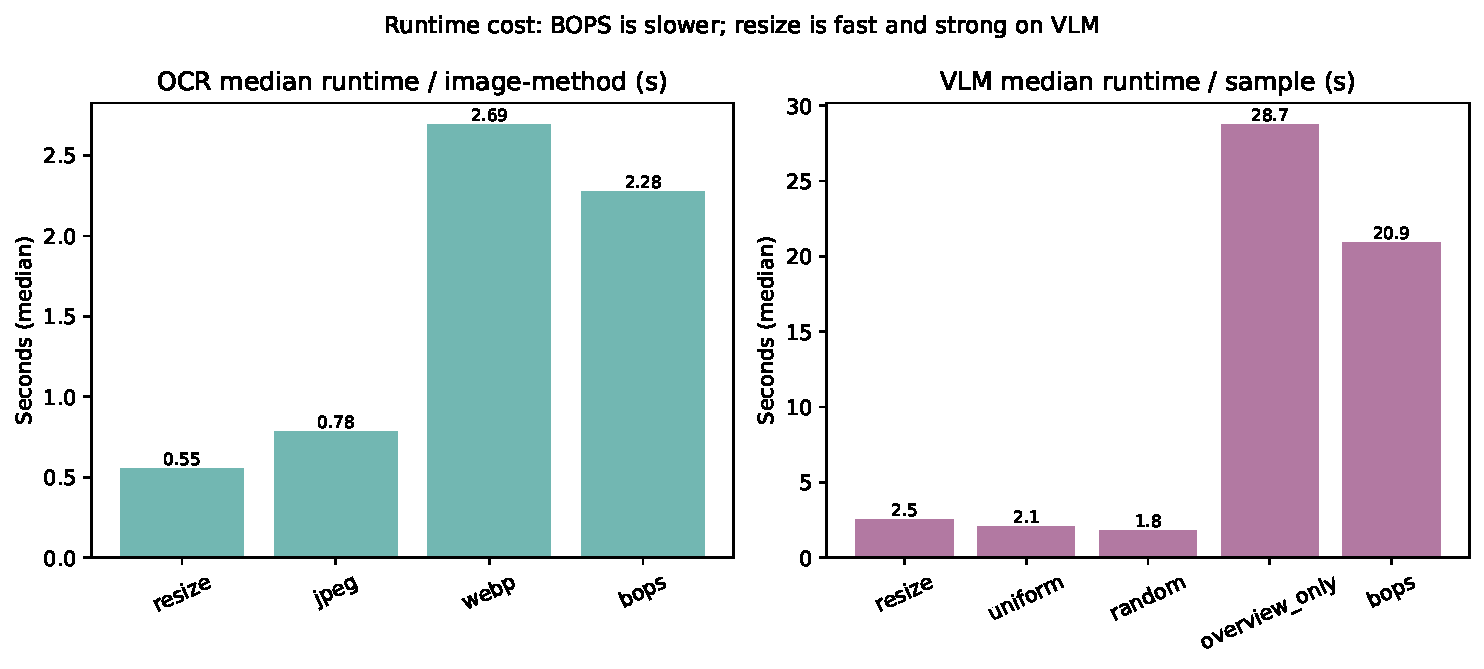
\includegraphics[width=\columnwidth]{figures/runtime_comparison.pdf}
    \caption{Median runtime comparison. BOPS has higher preprocessing/inference cost and does not currently outperform resize on DocVQA.}
    \label{fig:runtime}
\end{figure}

\begin{table*}[!ht]
\centering
\caption{Paired bootstrap confidence intervals for main comparisons.}
\label{tab:ci}
\begin{tabular}{llccc}
\toprule
Comparison & Metric & Mean diff. & 95\% CI & Significant \\
\midrule
BOPS p8 $-$ resize area 0.25 & word recall & +0.077 & [0.052, 0.102] & Yes \\
BOPS p8 $-$ original & word recall & -0.035 & [-0.054, -0.016] & Yes \\
BOPS $-$ random & ANLS & +0.036 & [-0.004, 0.083] & No \\
BOPS $-$ uniform & ANLS & -0.018 & [-0.088, 0.041] & No \\
BOPS $-$ overview-only & ANLS & +0.003 & [-0.048, 0.054] & No \\
\bottomrule
\end{tabular}
\end{table*}


\section{Discussion}
The results support three lessons. First, aggressive spatial resizing is harmful for OCR word recall, and high-resolution patches can recover text lost by strict downscaling. Second, byte compression is a strong OCR-preserving baseline and should be included in future visual-budget evaluations. Third, document QA is evidence-specific: preserving generally text-rich regions is not equivalent to preserving the region that answers a question.

This suggests that future patch selection should be question-aware. A simple next step is to score candidate patches not only by OCR density but also by similarity between OCR text inside a patch and the question tokens. This would still avoid answer leakage because the ground-truth answer is not used during patch selection.

\section{Threats to Validity and Limitations}
\textbf{Scale.} The experiments use 200 TextOCR images and 100 DocVQA questions. Larger samples are required for a full benchmark study.

\textbf{Single OCR and VLM backends.} OCR uses EasyOCR and VLM uses Qwen2.5-VL-3B. Results may change with other OCR engines or larger VLMs.

\textbf{Metric completeness.} Word recall alone can overstate OCR gains when patch merging adds noisy text; we therefore report word precision and F1. At patches 8, \method{} improves recall over resize area 0.25 but not F1 (0.199 vs.\ 0.193).

\textbf{Budget equivalence.} Area, byte, and patch budgets are not identical resource units. This study compares practical preprocessing strategies under declared budget axes rather than claiming perfect equivalence across all compute/token costs.

\textbf{Question-agnostic selection.} Current BOPS scoring does not use the question. This is the main reason VLM performance remains inconclusive.

\section{Conclusion}
This paper studied budget-aware preprocessing for text-rich image understanding. BOPS significantly improves OCR word recall over aggressive resizing on a 200-image TextOCR evaluation, but it does not significantly improve DocVQA performance on a 100-question VLM evaluation. Diagnostics show why: answer-bearing regions are often visible in full-image OCR but absent from the selected patches. The main research lesson is that OCR-guided patches can preserve text, but document question answering requires preserving question-specific evidence. A publishable next step is question-aware patch selection combined with larger-scale evaluation.

\balance
\bibliographystyle{IEEEtran}
\bibliography{references}

\appendices
\section{Supplementary Failure Examples}
\begin{figure*}[!ht]
    \centering
    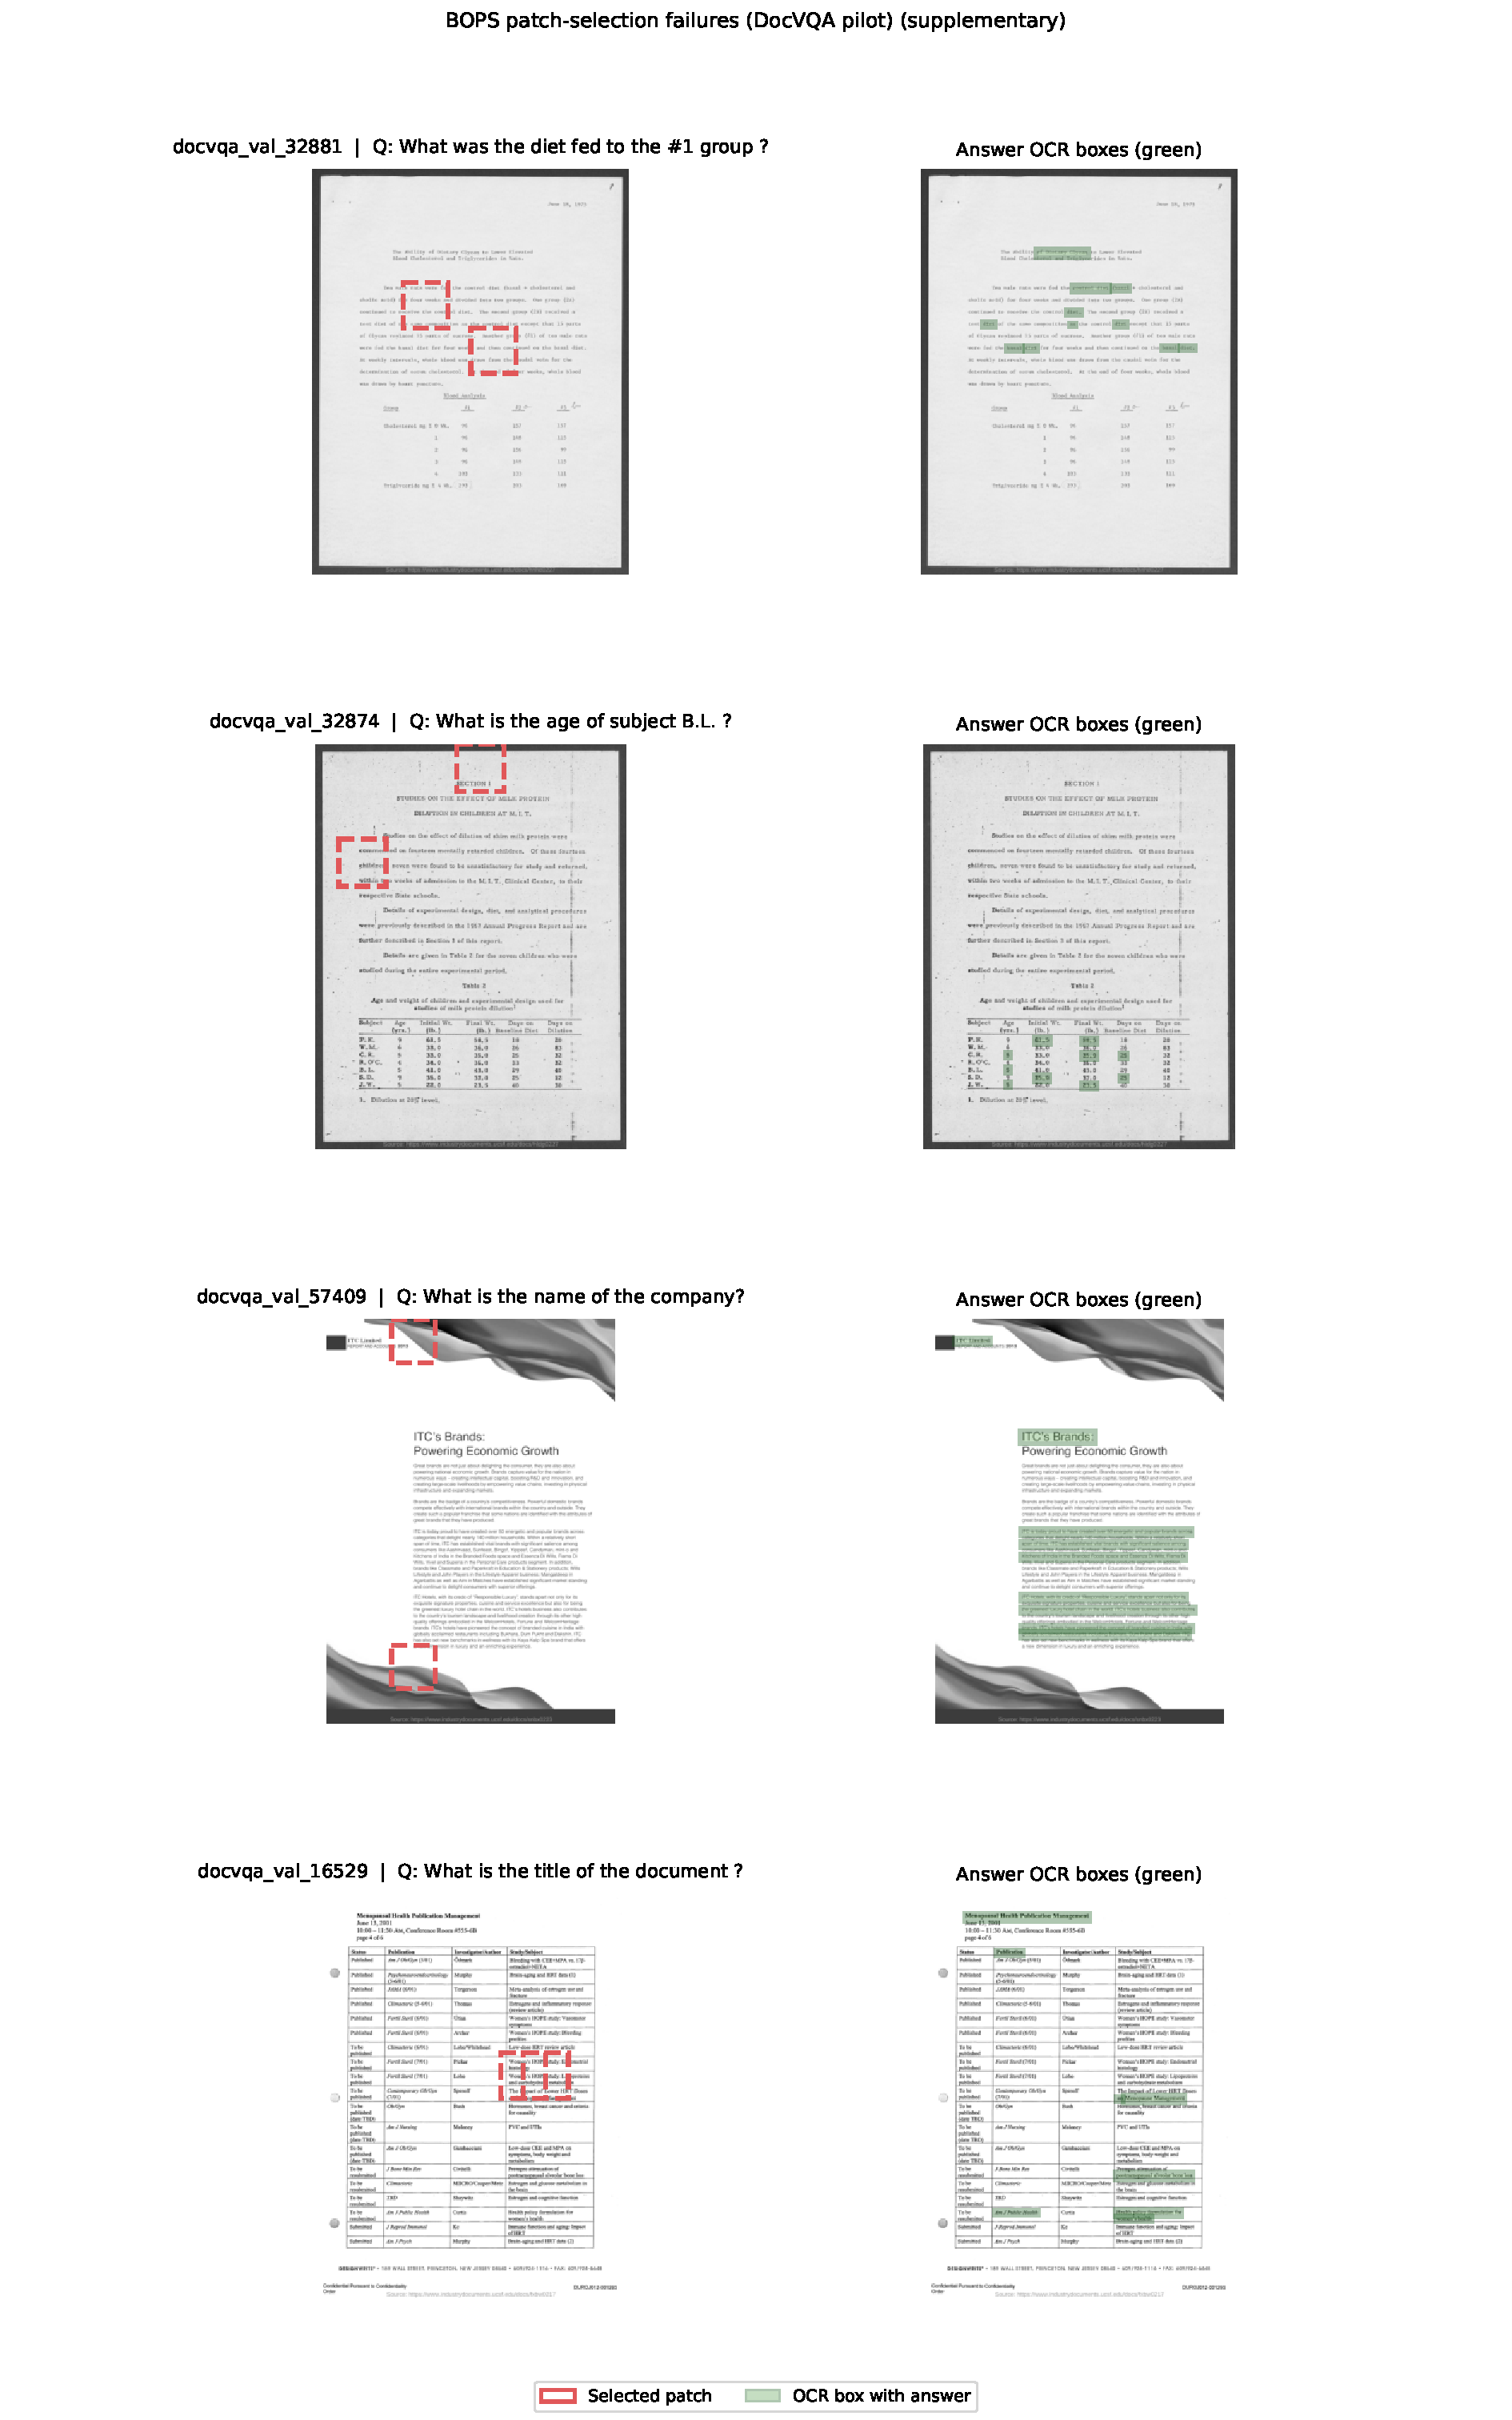
\includegraphics[width=0.92\textwidth]{figures/failure_panel_appendix.pdf}
    \caption{Additional BOPS patch-selection failures (supplementary material). Same ranking as Fig.~\ref{fig:failures}, excluding the main-paper example.}
    \label{fig:failures-appendix}
\end{figure*}

\end{document}
